\documentclass[12pt,a4paper]{report}

\title{Sistema de extracción automática de información de documentos}
\author{Daniel González Cerviño}
\date{\today}

% Configure languaje and codification
\usepackage[utf8]{inputenc}
\usepackage[spanish]{babel}
\selectlanguage{spanish}

% Image manipulation
\usepackage{graphicx}
\usepackage{tikz}
% Allow title personalization
\usepackage{titlesec}
% Allow use TrueType and Open Type fonts
\usepackage{fontspec}
\usepackage{lmodern}
% Allow use font colors
\usepackage{xcolor}
% Allow tables with 100% width
\usepackage{tabularx}
% Allow reference last page of document
\usepackage{lastpage}
% Allow advanded tools for headers and footers
\usepackage{fancyhdr}
% Allow references in APA style
\usepackage[style=apa, backend=biber]{biblatex}

% Allow insert notes
\usepackage{todonotes}

% Set margins
\usepackage[top=3.5cm,bottom=3.5cm,left=2.75cm,right=2.75cm,]{geometry}
\usepackage[T1]{fontenc}

% Set headers and footers
\fancypagestyle{plain}{%
    \renewcommand{\headrulewidth}{0pt}
    \fancyhead{}
    \fancyfoot{}
    \fancyfoot[R]
    {{ Sistema de extracción automática de información de documentos | \scriptsize\thepage\ de \pageref{LastPage}}}
    \fancyhead[L]
    {\tikz[remember picture,overlay]\node[opacity=0.4] at (-3mm, 10mm){
\includegraphics[scale=0.18]{./images/header}};}
    \fancyheadoffset{0pt}
}

% Define fonts
\setmainfont{Montserrat}
\newfontfamily\chapterfont{Oswald}
\newfontfamily\sectionfont{Oswald}

% Define colors
\definecolor{color_orange}{HTML}{E65113}
\definecolor{color_dark_grey_1}{HTML}{626262}
\definecolor{color_dark_grey_2}{HTML}{717171}

% chapter style format
\titleformat{\chapter}[hang]
{\chapterfont\Huge\bfseries\color{color_orange}}
{\thechapter}{1em}{}

% section style format
\titleformat{\section}[hang]
{\sectionfont\Large\bfseries\color{color_dark_grey_1}}
{\thesection}{1em}{}

% subsection style format
\titleformat{\subsection}{\sectionfont\large\bfseries\color{color_dark_grey_2}}{\thesubsection}{1em}{}

\pagestyle{plain}

\begin{document}

% cover
    \begin{titlepage}

    \tikz[remember picture,overlay]
    \node[opacity=1,inner sep=0pt] at (77mm, -110mm)
        {
\includegraphics{./cover/images/cover}};

    \vspace{50em}
    \fontspec{Oswald}[BoldFont={Oswald-Bold}]
    \fontsize{28}{10.4}\selectfont
    \color{white}
    \begin{flushleft}
        \textbf{Sistema de extracción de información de documentos}
    \end{flushleft}

    \restoregeometry
\end{titlepage}

    \noindent
\Huge\textbf{Trabajo final de grado}
\normalfont\normalsize
\vspace{3em}
\begin{table}[h]
    \renewcommand{\arraystretch}{1.5}
    \begin{tabular}{p{0.35\textwidth} p{0.65\textwidth}}
        \hline\textbf{Título}             & Sistema de extracción automática de información de documentos \\
        \hline\textbf{Universidad}  & Universidad Internacional de Valencia                         \\
        \hline\textbf{Titulación}   & Grado de ingeniería informática                               \\
        \hline\textbf{Mención}      & Ingeniería del software                                       \\
        \hline\textbf{Curso}        & 2023/24                                                       \\
        \hline\textbf{Convocatoria} & Primera convocatoria, Junio                                   \\
        \hline\textbf{Autor}        & Daniel González Cerviño, 49012312 W                           \\
        \hline\textbf{Directora}    & Marlene Goncalves Da Silva, Y7592198 G                        \\
        \hline
    \end{tabular}
    \label{tab:}
\end{table}


    \tableofcontents
    \addcontentsline{toc}{chapter}{\listfigurename}
    \addcontentsline{toc}{chapter}{\listtablename}
    \listoffigures
% Abstract
    \providecommand{\keywords}[1]
{
    \small
    \textbf{\textit{keywords: \hspace{0.3cm}}} #1
}
\begin{abstract}
    \todo[inline]{@TODO: completar al final}
    Es una sección concisa y precisa (400 a 500 palabras) que resume los aspectos más importantes del trabajo
    realizado. Su objetivo es proporcionar una visión general rápida y clara del contenido y los resultados obtenidos,
    capaz de captar la atención e interés del lector, invitándolo a leer el trabajo completo.
    El resumen debe comenzar con una breve introducción que contextualice el tema del trabajo y exponga la problemática
    abordada. Debes mencionar de manera breve los objetivos o propósitos principales del trabajo. Brevemente, describe
    los métodos/metodología o enfoque que has utilizado para llevar a cabo el trabajo. Resume los principales resultados
    obtenidos. Indica las conclusiones o contribuciones más importantes derivadas de tu trabajo.
    Palabras clave: Al final del resumen, proporciona una lista de palabras clave que representen los conceptos
    principales y los temas abordados en tu trabajo.

    \vspace{0.5cm}
    \keywords{primero, segundo, tercero}
\end{abstract}


% Dedication
    \newpage
\section*{Dedicatoria}

A Arancha, mi compañera incansable, cuyo apoyo ha sido fundamental en este proceso.
Gracias por asumir, con amor y sin quejas, la carga extra de nuestras responsabilidades familiares para que yo pudiera
concentrarme en este proyecto.
Tu fortaleza y dedicación son el cimiento de nuestra familia y de cada uno de mis logros.

A mis queridas hijas, Aroa y Enara, gracias por llenar cada día con vuestra alegría y vuestras ganas de vivir.
Vuestra energía y felicidad han sido la fuente de mis fuerzas y la luz en los momentos de oscuridad.
Os pido perdón por las veces que la consecución de este grado me ha apartado de vosotras, robándome momentos juntos.

Este trabajo es tan vuestro como mío.
Dedicado con todo mi amor y gratitud a las tres, por ser mi mayor inspiración y el motivo de mi esfuerzo.


%% Chapters
    \chapter{Introducción}\label{ch:chapter_1}


\section{Antecedentes}

El desarrollo de este Trabajo de Fin de Grado (TFG) surge de una necesidad surgida en mi faceta profesional, donde la
tarea repetitiva de leer y extraer información de documentos representa una carga significativa para la empresa en la
que trabajo.

Este desafío no es exclusivo de mi actual empresa actual, sino que es una realidad común en una variedad de sectores
incluyendo entre otros:

\begin{itemize}
    \item Compañías de seguros
    \item Instituciones educativas
    \item Empresas del sector sanitario
    \item Empresas de gestión de recursos humanos
    \item Entidades financieras
\end{itemize}

Estas organizaciones enfrentan el reto constante de gestionar grandes volúmenes de documentación, lo cual resalta la
importancia y la necesidad universal de soluciones automatizadas que permitan extraer información de los mismos.

Durante la asignatura del Grado de Ingeniería Informática 47 Proyecto de Ingeniería del Software, tuve la oportunidad de
desarrollar una base técnica preliminar que se ha convertido en la base para la realización de este proyecto.


\section{Planteamiento del problema}

Estas tipologías de empresas que hemos visto en el apartado anterior se enfrentan a la necesidad de procesar una enorme
cantidad de documentos.

Por ejemplo una empresa que gestiona seguros de coche, deberá recibir un paquete de datos de cada nuevo cliente que
contendrá entre otros los siguientes documentos: documento de identidad del titular y los tomadores, carne de conducir
de los tomadores, ficha técnica del vehículo,permiso de circulación, recibo del impuesto de vehículo de tracción
mecánica.

La forma tradicional de obtener la información de dichos documentos consiste en que un operario reciba los datos y los
introduzca en el sistema.
Esta metodología tradicional enfrenta una problemática significativa:

\begin{itemize}
    \item \textbf{Elevado coste financiero}
    El personal dedicado a estas tareas genera un gasto que impacta directamente en el coste operativo de la
    organización
    \item \textbf{Demora en los tiempos de tramitación}
    La tramitación manual implica que los documentos no van a ser procesados en el tiempo en que son recibidos, sino
    que deberán esperar a que un operario esté disponible para ocuparse de esta tarea
    \item \textbf{Pobre asignación de recursos}
    Los recursos invertidos en la operación manual de documentos podrían ser mejor asignados a actividades que aporten
    valor real a la organización
    Esto incluye tareas que potencian la innovación, el desarrollo estratégico y el servicio al cliente, entre otros
    \item \textbf{Incidencia de errores manuales}
    La tramitación manual de documentos es intrínsecamente susceptible a errores humanos
\end{itemize}

Ante esta situación, se hace necesario el desarrollo de soluciones tecnológicas que automatizan y optimizan el proceso
de extracción de la información.


\section{Justificación}

La relevancia de este TFG se fundamenta en la necesidad de implementar soluciones tecnológicas que automaticen la
extracción de la información contenida en documentos.

\begin{itemize}
    \item
    Desde el punto de vista profesional este proyecto responde a una necesidad práctica de desarrollar una solución
    que permita la recuperación de la información contenida en diferente tipo de documentos.
    \item Desde la perspectiva académica, el desarrollo de un sistema de extracción automática de información aborda
    competencias clave en la ingeniería informática, tales como la programación, el análisis de sistemas, y
    especialmente, el procesamiento de lenguaje natural y la inteligencia artificial.
\end{itemize}

En resumen, este TFG no solo es una oportunidad para aplicar habilidades y conocimientos técnicos adquiridos durante el
grado, sino también una contribución valiosa a la innovación de sistemas digitales en mi ámbito profesional.


\section{Objetivos}

El propósito central de este trabajo es la creación de un sistema que permita la extracción automática de documentos.

Como este objetivo puede resultar demasiado ambicioso, el alcance de este TFG quedará limitado a los siguientes
objetivos específicos.
Los objetivos específicos incluyen:

\begin{enumerate}
    \item
    Desarrollar un sistema capaz de convertir documentos PDF en documentos de texto plano que puedan ser procesados.
    \item Implementar dos casos de uso dentro del sistema:
    \begin{enumerate}
        \item Contratos de alquiler de vivienda entre particulares
        \item Contratos de compraventa de vehículos entre particulares
    \end{enumerate}
    \item Diseñar una interfaz que permita a los usuarios interactuar con este sistema.
    \item Evaluar la eficacia del sistema mediante un conjunto de pruebas
\end{enumerate}

\begin{figure}[ht]
    \begin{center}
        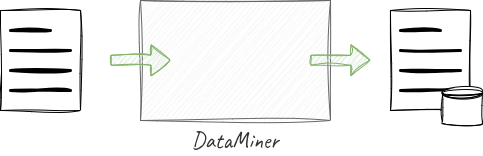
\includegraphics[scale=0.5]{./chapter/images/chapter_1.overview}
        \caption{Esquema general del sistema. \textit{Elaboración propia.}}
        \label{fig:chapter_1.overview}
    \end{center}
\end{figure}

\todo[inline]{@TODO: Mejorar la figura}

Tal y como se puede ver en la figura \ref{fig:chapter_1.overview}
el sistema recibe documentos y genera información en un formato estructurado.
El tipo de estructura, dependerá del tipo de documento.
Por ejemplo en un contrato de alquiler de vivienda aparecerán los datos de la vivienda, y en un contrato de compraventa
de vehículos, aparecerán los datos del vehículo.

    \chapter{Marco teórico}\label{ch:chapter_2}

\todo[inline]{@Marlene: colocas definiciones en las secciones pero no las referencias de esas definiciones
También debes relacionar cada seccion con tu trabajo Código limpio y arquitectura limpia pueden ir en una sola seccion
Si colocas una figura, debes referenciarla en el texto y explicarla}


\section{Código limpio}

\subsection{Introducción histórica}
El concepto de Código Limpio ha sido fundamental en la programación de software desde los primeros días del desarrollo
de software, pero fue articulado y popularizado con gran efecto por Robert C. Martin en su libro~\cite{book_martin_2008}

Este libro se convirtió en una guía esencial para muchos desarrolladores al enfatizar la importancia de escribir código
que no solo funcione, sino que también sea fácil de entender, modificar y mantener.

\subsection{Definición}
Código limpio es aquel que es fácil de entender y fácil de modificar.
Es elegante, eficiente y hace exactamente lo que se espera que haga.
Según Robert C. Martin, el código limpio puede ser leído y mejorado por un
desarrollador que no sea su autor original con un mínimo esfuerzo necesario.

Se caracteriza por su simplicidad, la ausencia de duplicación, la expresión clara de la intención del desarrollador, y
la atención a los detalles en el nivel de código.
Contiene los tests, no contiene errores y, lo más importante, revela claramente su diseño y propósito.


\section{Arquitectura limpia}

\subsection{Introducción histórica}
En el ámbito del desarrollo de software, la estructuración eficiente de la arquitectura de un sistema
es crucial para determinar su eficiencia, escalabilidad y mantenibilidad a largo plazo.

Una de las metodologías que ha cobrado relevancia en este contexto es la Arquitectura Limpia,
un enfoque sistemático para el diseño de software promovido por
Robert C. Martin.
En su libro Clean Architecture: A Craftsman\'
s Guide to Software Structure and Design (Martin, 2017), Martin presenta un marco de trabajo que prioriza la separación
de preocupaciones y la independencia de los diversos componentes del software.

\subsection{Definición}
La arquitectura limpia es un estilo de diseño de software que
organiza el sistema de manera que sea independiente de frameworks, UI, bases de datos y cualquier otra agencia externa.

\todo[inline]{@TODO: Insertar figura}
\todo[inline]{@Marlene: hay que referenciar en el texto la figura. Te falta colocar la referencia}

Representación de las comunicaciones entre capas en una arquitectura limpia.

La esencia de esta arquitectura radica en su diagrama concéntrico de capas, donde cada capa tiene responsabilidades
claramente definidas y depende solo de las capas más internas.
Esto se logra mediante el principio de Inversión de dependencias, lo que significa que los detalles dependen de las
abstracciones y no al contrario.

Aunque existen diferentes implementaciones de una arquitectura limpia, cada una con sus características intrínsecas, en
este proyecto hemos decidido implementar una versión en 3 capas.

\todo[inline]{@Marlene: mencionales. Aparecen 4 a continuación, por qué?}
\subsubsection*{Dominio}
Es el corazón del modelo de negocio de la aplicación y encapsula la
lógica y las reglas del negocio.

Esta capa es fundamentalmente agnóstica respecto a la aplicación de tecnologías externas y se
centra exclusivamente en cómo se comporta el negocio bajo diferentes condiciones y reglas.

Contiene entidades, objetos de valor, y dominios de servicio que representan y operan sobre los
conceptos fundamentales del negocio.

Esta capa debe ser autocontenida y fácilmente testable, aislada de influencias externas como bases de
datos o interfaces de usuario.

\subsubsection*{Aplicación}
La capa de aplicación actúa como un mediador entre la capa de presentación y la capa de dominio, coordinando
las operaciones de alto nivel que involucran múltiples aspectos del dominio.

\subsubsection*{Infraestructura}
La capa de infraestructura proporciona las capacidades tecnológicas necesarias para que las capas de
aplicación y dominio puedan realizar sus funciones sin tener que
preocuparse por los detalles de implementación de la plataforma o los elementos externos.

\subsubsection*{Presentación}
Es responsable de mostrar la información al usuario y de interpretar los
comandos del usuario para que la aplicación pueda entenderlos y actuar en consecuencia.

\todo[inline]{@Marlene: queda mejor si lo redactas como parrafo y no siguiendo ese estilo}


\section{Procesamiento de lenguaje natural}

\subsection{Introducción histórica}
El Procesamiento de Lenguaje Natural o Natural Language Processing (NLP) es un campo que se sitúa en la
intersección de la informática, la inteligencia artificial y la lingüística.

Se dedica al desarrollo de algoritmos y sistemas que permiten a las computadoras entender, interpretar y generar
lenguaje humano de una manera útil y significativa.
La historia del NLP comienza en la década de 1950, marcada por el trabajo pionero de Alan Turing y su famoso
test de Turing, que planteaba la cuestión de si una máquina puede emular el lenguaje humano de manera convincente
(Turing, 1950).

En los años 60 y 70, el enfoque inicial en la traducción automática
, como los esfuerzos del proyecto Georgetown, mostró tanto promesas como limitaciones significativas, lo que llevó a un
reajuste en las expectativas y métodos del campo (Hutchins, 2003).
Con la introducción de la inteligencia artificial (IA) en la década de 1980, surgieron métodos basados primero en reglas
y luego en modelos
estadísticos, culminando con el desarrollo de modelos de aprendizaje automático en la década de 1990 (Manning y Schütze,
1999).

El verdadero cambio paradigmático llegó con el advenimiento de las redes neuronales y el aprendizaje profundo
en la década de 2010.
Este período vio la creación de modelos de lenguaje avanzados, como BERT y GPT, que han revolucionado la capacidad de
las máquinas para procesar el lenguaje con un grado de sutileza y profundidad sin precedentes (Devlin et al., 2019;
Brown et al., 2020).

\subsection{Definición}
El NLP es un campo que combina técnicas de la informática, la inteligencia artificial y la lingüística computacional con
el objetivo de permitir que las máquinas entiendan, interpreten
, manipulen y generen lenguaje humano de manera efectiva y eficiente.

El NLP utiliza algoritmos y modelos matemáticos para abordar diversas tareas relacionadas con el lenguaje, tales como la
traducción automática entre idiomas, la generación de respuestas automáticas
, la extracción de información relevante de textos, el análisis de sentimientos, el reconocimiento de voz, y
la síntesis de habla, entre otros.


\section{Modelos de lenguaje de gran escala (LLMs)}

\subsection{Introducción histórica}
La historia de los LLMs comienza con los primeros modelos estadísticos de lenguaje en
la década de 1980, que utilizaban métodos simples como los modelos de Markov y n-gramas para predecir la probabilidad
de secuencias de palabras (Jelinek, 1997).
Estos métodos, aunque efectivos para algunas tareas básicas, estaban limitados por su incapacidad para capturar
contextos
más largos y por su dependencia de grandes corpus de texto para entrenamiento.

En la década de 2000, con el advenimiento de modelos más sofisticados como los modelos ocultos de Markov
y especialmente las redes neuronales, comenzó a vislumbrarse el
potencial de los modelos de lenguaje más complejos.
Sin embargo, no fue hasta la introducción de las redes neuronales recurrentes (RNN) y, más tarde, las redes neuronales
de memoria a largo plazo (LSTM)
que los investigadores pudieron abordar el problema del ''desvanecimiento del gradiente''
y mejorar significativamente la capacidad de los
modelos para aprender dependencias a largo plazo en el texto (Hochreiter Schmidhuber, 1997).

\subsubsection*{La revolución de los transformers}
El verdadero cambio paradigmático llegó en 2017 con el desarrollo de la arquitectura
Transformer por Vaswani et al.
Esta arquitectura introdujo el mecanismo de atención, que permite a los modelos ponderar diferentes partes de la entrada
de texto de manera dinámica, mejorando la capacidad de los modelos para manejar secuencias de texto largas y complejas (
Vaswani et al., 2017).

\todo[inline]{@Marlene: Transformers términos en inglés van en itálicas}

BERT, desarrollado por Google en 2018, y GPT, desarrollado por OpenAI, son ejemplos de
cómo los Transformers han sido adaptados para crear modelos que
no solo entienden el contexto de una palabra en función de su posición en una frase, sino en todo
el texto, permitiendo un entendimiento contextual mucho más rico (Devlin et al., 2019; Radford et al., 2018).

\subsection{Definición}
Los Modelos de Lenguaje de Gran Escala (LLMs) son sistemas
avanzados de inteligencia artificial diseñados para entender, generar y
manipular el lenguaje humano de manera coherente y contextualizada. Estos
modelos son entrenados en vastos conjuntos de datos textuales que abarcan una amplia variedad de temas, lo que les
permite desarrollar un conocimiento extenso sobre el lenguaje y sus usos prácticos.

Funcionan principalmente a través de técnicas de aprendizaje
profundo, especialmente usando arquitecturas como las de Transformers,
que permiten a los modelos captar relaciones complejas y contextos a largo plazo dentro de los textos. Este enfoque les
otorga la capacidad de generar respuestas, completar textos,
traducir entre idiomas, resumir información y responder preguntas con un alto grado de precisión y relevancia.

\subsection{Principales modelos}

\todo[inline]
{@Marlene: puedes hacer un resumen de estos modelos. Creo que no hace falta que coloques los código de ejemplos. Quizás
para un anexo}
\subsubsection*{OpenAI GPT}
ChatGPT es un avanzado modelo de lenguaje desarrollado por OpenAI,
basado en la arquitectura GPT (Generative Pre-trained Transformer).

Es uno de los modelos más reconocidos en la actualidad.
Aunque es un modelo privado, OpenAI ofrece acceso a través de una API de pago que incluye una capa gratuita limitada.

ChatGPT ofrece varios modelos, cada uno con un esquema de precios que varía según
su complejidad.
Una de las principales ventajas de este servicio es que proporciona una solución integral "plug-and-play", es decir, no
requiere instalación ni configuración adicional por parte del usuario.

A continuación un ejemplo de una llamada a esta API.


\subsubsection*{Hugging Face's Transformers}
Hugging Face's Transformers
es una biblioteca de procesamiento de lenguaje natural (NLP) que simplifica el uso de modelos de aprendizaje profundo
basados en la arquitectura Transformer.

Esta biblioteca ofrece una amplia variedad de modelos pre entrenados desarrollados por la comunidad
para fines específicos, además de la posibilidad de entrenar modelos personalizados.


Sin embargo, los modelos disponibles en Hugging Face suelen ser menos potentes que los modelos más
avanzados disponibles a través de plataformas como ChatGPT. ChatGPT ofrece
modelos con capacidades superiores, lo que puede ser una
consideración importante dependiendo de los requisitos específicos del proyecto.

\subsubsection*{Otros}
Además de OpenAI y Hugging Face, existen varias otras plataformas que ofrecen modelos de lenguaje
grande (LLM) para desarrolladores interesados en incorporar capacidades
avanzadas de procesamiento de lenguaje natural en sus aplicaciones. Entre
estas plataformas destacan Google AI, Facebook AI, NVIDIA NeMo y Microsoft AI, entre otras cada una con sus propios
enfoques y modelos distintivos.

    \chapter{Desarrollo}\label{ch:chapter_3}


\section{Descripción del proyecto}

Hemos creado una solución tecnológica con dos interfaces una web y una de línea de comandos, que transforma los datos no
estructurados de documentos PDF en formatos estructurados y utilizables.


\section{Alcance}

El software que hemos desarrollado hasta ahora sirve como una base conceptual y prototipo inicial.

Se ha desarrollado una herramienta que es capaz de procesar datos de contratos de los siguientes tipos

\begin{enumerate}
    \item Contrato de arrendamiento de vivienda
    \item Contrato de compraventa de vehículo entre particulares
\end{enumerate}

Aunque ha demostrado la viabilidad de la idea, aún requiere validación extensiva y mejoras antes de que esté listo para
su implementación en entornos de producción real.

Nuestro próximo objetivo es abrir el proyecto a la comunidad, convirtiéndolo en una iniciativa de código abierto.

Esto no solo incluirá la mejora y ampliación de la documentación existente, sino también la traducción al inglés para
facilitar su adopción y contribución global.
Además, planeamos desarrollar más funcionalidades y realizar pruebas exhaustivas para asegurar la robustez y fiabilidad
del software.


\section{Metodología de desarrollo}

Nuestro proyecto se ha desarrollado utilizando la metodología Extreme
Programming (XP), una metodología ágil que enfatiza la adaptabilidad y la colaboración del equipo (Beck, 2000).

Hemos adoptado prácticas como la integración continua y el desarrollo orientado a pruebas para mejorar la
calidad del código y la respuesta a los cambios (Fowler \& Foemmel, 2006).

Hemos gestionado el flujo de trabajo utilizando un tablero Kanban en GitHub Projects, lo que ha permitido un seguimiento
visual y eficiente del progreso (Anderson, 2010).


\section{Tecnologías utilizadas}
El proyecto hace uso de una variedad de tecnologías modernas para asegurar un desarrollo eficiente,
una implementación robusta y una experiencia de usuario óptima.

A continuación, se describen las principales tecnologías utilizadas en
el proyecto, categorizadas en distintas áreas según su propósito y aplicación.

\subsection{Backend}

*PHP

Es un lenguaje de scripting de propósito general que está especialmente diseñado para el desarrollo web.
PHP permite crear aplicaciones web dinámicas y está ampliamente soportado en servidores web.

Symfony

Symfony es un framework PHP ampliamente utilizado para desarrollar aplicaciones web.
Ofrece una arquitectura robusta y flexible, que facilita el desarrollo de aplicaciones mantenibles y escalables.

Twig

Twig es un motor de plantillas para PHP, utilizado principalmente en proyectos basados en
Symfony.
Facilita la creación de vistas dinámicas y mantenibles, separando la lógica de presentación del código de negocio.

\subsection{Frontend}

HTML5

Es el estándar de marcado para crear páginas web.
HTML5 introduce nuevas funcionalidades como elementos semánticos y multimedia, mejorando la accesibilidad y la
interoperabilidad de las páginas web.

CSS3

Es la tecnología de estilos para el diseño visual.
CSS3 permite aplicar estilos complejos y responsivos a los elementos HTML, mejorando la presentación y la experiencia
del usuario.

JavaScript

Es el lenguaje de programación para la interactividad del lado del cliente.
JavaScript permite crear experiencias de usuario dinámicas y responsivas, manejando eventos y actualizando el contenido
de la página sin recargar.

Bootstrap

Es un framework de front-end que facilita el diseño de sitios y aplicaciones web
responsivas y móviles.
Bootstrap proporciona una colección de componentes CSS
y JavaScript predefinidos que aceleran el desarrollo de interfaces de usuario atractivas.

Font Awesome

Es una biblioteca de iconos vectoriales y herramientas que proporciona una amplia gama de
iconos escalables y personalizables para su uso en proyectos web.
Facilita la inclusión de iconos de alta calidad sin depender de imágenes.

\subsection{Gestión de dependencias}

Composer

Es una herramienta de gestión de dependencias para PHP, que
permite declarar las bibliotecas de las que depende tu proyecto
y las gestiona.
Composer asegura que las versiones correctas de las bibliotecas se instalen y mantengan actualizadas.

\subsection{Control de versiones}

Git

Es un sistema de control de versiones distribuido, diseñado para manejar todo, desde proyectos
pequeños hasta muy grandes con rapidez y eficiencia.
Git permite a los desarrolladores colaborar de manera efectiva, rastreando cambios y gestionando ramas y fusiones.


GitHub

GitHub es una plataforma de hospedaje de repositorios Git.
Proporciona herramientas para la colaboración, la revisión de código y la gestión de proyectos, facilitando el trabajo
en equipo y la integración continua.

\subsection{Automatización}

Make

Make es una herramienta de automatización de tareas que utiliza archivos Makefile para definir y ejecutar tareas de
construcción y gestión de proyectos.
Facilita la automatización de tareas repetitivas y la configuración del entorno de desarrollo.

\subsection{Pruebas}

PHPUnit

PHPUnit es un marco de pruebas unitarias para PHP. Permite a los desarrolladores escribir y ejecutar pruebas
automatizadas
para asegurar que el código se comporta como se espera, facilitando el desarrollo de software de alta calidad.

GitHub Actions

Es una plataforma de integración continua que permite automatizar flujos de trabajo directamente desde GitHub.
GitHub Actions facilita la configuración de pipelines de CI/CD, ejecutando pruebas y despliegues automáticamente con
cada cambio en el repositorio.

\subsection{Contenerización}

Docker

Docker es una plataforma que permite desarrollar, enviar y ejecutar aplicaciones dentro de
contenedores.
Proporciona un entorno consistente para el desarrollo, pruebas y despliegue, asegurando que las aplicaciones funcionen
de manera idéntica en diferentes entornos.

Docker Compose

Docker Compose es una herramienta para definir y ejecutar aplicaciones Docker multi-contenedor.
Permite orquestar varios servicios que componen una aplicación, facilitando
la configuración y gestión de entornos de desarrollo complejos.

\subsection{Logs}

Monolog

Monolog es una biblioteca de logging para PHP. Permite enviar registros a varios destinos, como archivos, bases de datos
y servicios de terceros, facilitando la monitorización y depuración de aplicaciones.

Elastic Search

Elasticsearch es un motor de búsqueda y análisis de texto completo basado en Lucene.
Permite almacenar, buscar y analizar grandes volúmenes de datos en tiempo real.

Logstash

Logstash es una herramienta de procesamiento de datos que ingesta, transforma y envía datos a varios
destinos.
Es parte del paquete Elasticsearch, Logstash, Kibana (ELK) y facilita la recolección y procesamiento de logs.

Kibana

Kibana es una herramienta de visualización de datos que trabaja en conjunto con Elasticsearch.
Permite a los usuarios crear gráficos y dashboards interactivos para visualizar y analizar los datos de logs almacenados
en Elasticsearch.

\subsection{Componente Generator}

Pdf to text

Pdf to Text es una herramienta que convierte documentos PDF en texto plano.
Permite extraer el contenido textual de archivos PDF, lo cual es útil para la posterior manipulación y análisis de
datos.

\subsection{Componente Reader}

Symfony HttpClient

Symfony HttpClient es un cliente HTTP flexible y eficiente para PHP. Permite realizar solicitudes HTTP a servicios
externos, manejar respuestas y gestionar errores de manera sencilla y eficaz.

Symfony Cache

Symfony Cache es un componente de Symfony que proporciona una implementación robusta y flexible para el almacenamiento
en caché.
Permite mejorar el rendimiento de la aplicación mediante el almacenamiento temporal de datos, reduciendo la carga en los
recursos externos.

API Open AI

La API de OpenAI proporciona acceso a modelos avanzados de procesamiento de lenguaje natural.
Permite integrar capacidades de IA en la aplicación, como la generación de texto y el análisis de datos, mejorando las
funcionalidades y experiencias del usuario.

    \chapter{Resultados}\label{ch:chapter_4}


\section{Descripción de la solución}
El sistema desarrollado consta de una arquitectura basada en dos componentes principales: Generator y Reader.

Ambos componentes están diseñados para ser fácilmente extensibles, mediante un sistema en el que se pueden registrar
nuevos pre procesadores, procesadores y post procesadores, para cumplir con los requisitos de casos de uso específicos.

\subsection{Componente Generator}
El componente Generator se encarga de convertir documentos en diferentes formatos a texto plano.
En esta implementación, se desarrolló un procesador especializado que utiliza la herramienta pdftotext para transformar
documentos PDF en texto.

La arquitectura modular del Generator permite la inclusión de nuevos pre procesadores y post procesadores para ajustar y
perfeccionar el texto generado.

\subsection{Componente Generator}
El componente Reader interpreta y extrae la información estructurada del texto generado por el Generator.

Funciona mediante un sistema de procesadores organizados en una única capa, que opera bajo un mecanismo competitivo
similar al del componente Generator.
Los procesadores compiten entre sí para determinar cuál es el más adecuado para analizar y extraer la información
necesaria del texto.

En esta implementación, se desarrollaron dos procesadores que consumen la api pública de OpenAI, para extraer la
información de dos tipos de contratos diferentes: contratos de arrendamiento entre particulares y contratos de
compraventa de vehículos entre particulares.

\subsection{Interfaces de Usuario}
Para interactuar con el sistema, se han desarrollado dos interfaces:

\begin{itemize}
    \item Interfaz de Línea de Comandos: Esta herramienta está dirigida a desarrolladores y
    administradores del sistema, permitiendo ejecutar comandos y scripts directamente.


    \item Interfaz Web: Presenta un área donde los usuarios pueden
    arrastrar y soltar documentos para su análisis y muestra una representación en formato JSON de la información
    extraída.
\end{itemize}


\section{Pruebas y análisis de los resultados}

// @TODO, explicar de nuevo que seha desarrollado una test suite de pruebas unitarias, y
completar indicando el porcentaje de acierto para las pruebas manuales.

Resultados cuantitativos: Presenta los resultados numéricos o medibles de tu
proyecto.
Esto puede incluir métricas de rendimiento, tiempos de respuesta, velocidad de procesamiento, eficiencia,
precisión, entre otros.
Utiliza tablas, gráficos u otros medios visuales para mostrar claramente los datos recopilados.

Resultados cualitativos: Si tu proyecto implica evaluaciones subjetivas o cualitativas, como la usabilidad, la
experiencia del usuario o la calidad percibida,describe los resultados obtenidos a través de encuestas, entrevistas o
pruebas de usabilidad.

Pruebas y resultados funcionales: se presentan los resultados de las pruebas realizadas para verificar el correcto
funcionamiento de la solución.

Muestra cómo se han llevado a cabo las pruebas y los casos de prueba utilizados.
Destaca los resultados obtenidos en términos de la funcionalidad y el cumplimiento de los requisitos establecidos.

Casos de estudio o resultados específicos: Si has realizado estudios de casos específicos o evaluaciones particulares,
describe los resultados obtenidos y su relevancia para tu proyecto.
Puedes incluir ejemplos concretos de cómo la solución informática ha sido aplicada en situaciones reales y los
resultados obtenidos en cada caso.

Validación y pruebas: Explica cómo se han validado y evaluado los resultados de tu proyecto.
Si has realizado pruebas, verifica que se cumplan los requisitos establecidos y describe cómo se ha llevado a cabo la
evaluación.
Si se han utilizado conjuntos de datos de prueba o casos de uso específicos, menciónalos en esta sección.

Comparación con resultados esperados: Compara tus resultados con los objetivos
y las expectativas establecidos en la introducción de tu trabajo.
Destaca si has logrado alcanzar tus metas y si los resultados obtenidos son consistentes con las hipótesis o
predicciones iniciales.
Si hay desviaciones o discrepancias, explícalas y proporciona posibles explicaciones.

Análisis de los resultados: Realiza un análisis de los resultados obtenidos y su relevancia para tu proyecto.


\section{Rendimiento}

// @TODO: Rendimiento y eficiencia: evaluación del rendimiento y la eficiencia de la solución informática.
Muestra los resultados obtenidos en términos de tiempos de respuesta,velocidad de procesamiento, uso de recursos,
escalabilidad, entre otros aspectos relevantes para tu proyecto.
Compara los resultados con los objetivos establecidos.


\section{Calidad del código}

// @TODO, Calidad del código y mantenibilidad:
Evalúa la calidad del código desarrollado y la mantenibilidad de la solución.


\section{Limitaciones}

// @TODO, Limitaciones y posibles mejoras: Menciona las limitaciones o restricciones
que puedan haber afectado sus resultados.
Esto puede incluir limitaciones en los datos, en los métodos utilizados o en la implementación del proyecto.
También puedes sugerir posibles mejoras o áreas de investigación futuras basadas en las limitaciones identificadas.


\section{Coste}
// @TODO,


\section{Posibles mejoras}

\subsection{OCR}
// @TODO:

\subsection{Nuevos Readers}
// @TODO:

    \chapter{Conclusiones}\label{ch:chapter_5}


Este apartado resume los hallazgos, los logros y las implicaciones de tu trabajo.
A continuación, se presentan algunos elementos típicos que se deben incluir:

Recapitulación de los objetivos: Repasa brevemente los objetivos establecidos al comienzo del y evalúa en qué medida se
han logrado.

Destaca los principales resultados y contribuciones de tu proyecto.

Síntesis de los resultados: Resume los resultados más importantes y relevantes obtenidos durante el desarrollo.

Implicaciones y relevancia: Discute las implicaciones de tus resultados y su relevancia para el campo
de la ingeniería informática.
Explica cómo tus hallazgos contribuyen al conocimiento existente o tienen aplicaciones prácticas.
Destaca el valor y la importancia de tu trabajo.

Reflexión sobre el proceso de desarrollo: Realiza una reflexión sobre el proceso de desarrollo de tu proyecto y evalúa
su eficacia.
Identifica las fortalezas y las limitaciones de tu enfoque y ofrece recomendaciones para futuros proyectos similares.
Describe cualquier desafío o dificultad que hayas enfrentado durante el desarrollo y cómo los has abordado.

Cumplimiento de los requisitos y objetivos: Evalúa en qué medida tu solución cumple con los requisitos y objetivos
establecidos al inicio de tu proyecto.
Destaca los aspectos en los que has logrado cumplir plenamente los requisitos y aquellos en los que has encontrado
limitaciones o mejoras potenciales.

Lecciones aprendidas: Comparte las lecciones aprendidas durante tu trabajo y desarrollo.
Destaca las habilidades y conocimientos adquiridos, así como los aspectos que te han permitido crecer como ingeniero
informático.
Reflexiona sobre los desafíos, los éxitos y los obstáculos superados durante el proyecto.

Trabajo futuro: Proporciona sugerencias y recomendaciones para futuros trabajos o investigaciones en el campo.
Identifica áreas que requieren una mayor exploración, mejoras adicionales o extensiones de tu trabajo actual.

Las conclusiones deben ser claras, concisas y basadas en los resultados y la evidencia presentada en tu trabajo.
Evita introducir nueva información en esta sección y enfócate en
resumir los aspectos más destacados y significativos de tu trabajo.


\section{Iteraciones y mejoras}
// @TODO:

Si has realizado iteraciones o mejoras en el proceso de desarrollo, menciona los cambios realizados y las razones detrás
de ellos.


\section{Rubrica}
// @TODO: Revisar al rubrica.



%% Anexos
%    \appendix
%    \chapter{Instrucciones adicionales}\label{ch:appendix_1}


El apéndice es toda la información adicional complementaria, necesaria para ilustrar mejor el cuerpo del trabajo.

Los apéndices van numerados con una secuencia alfabética de letras mayúsculas (A, B, C, etc.). En caso de que se hayan
producido diagramas de clases, diagramas de la base de datos, casos de usos u otra información gráfica y estos no hayan
sido incluidos como parte del cuerpo del trabajo, deberán ser incluidos en la sección de apéndices.

Apéndice A

Ejemplos formatos
El estilo del párrafo tiene que ser encuadrado (justificado).
En caso de terminar con un apartado (nivel uno de título) aplicar un salto de página para comenzar siempre el siguiente
apartado en una página nueva.

Tablas

Tanto las figuras como las tablas tienen que estar indicadas en el texto y referenciadas con la numeración que tiene
asignada.
La descripción debe ser clara y explicar lo que se quiere representar con independencia de la referencia del texto.

Tanto las tablas como las figuras tendrán un estilo de párrafo centrado.
La descripción se realizará desde “Insertar título”.


Tabla 1. Operaciones matemáticas utilizadas en el estudio realizado. Elaboración propia.

Figuras

Las figuras deben estar mencionadas en el texto y ser referenciadas por su numeración Ejemplo: Se habilita un servidor
con Jupyter como se puede ver en la Figura 1, en el cual se puede disponer de diferentes kernels de programación
(Python, R, Julia…).

Figura 1.
Arquitectura Jupyter Cliente - Servidor.
Fuente: https://www.paradigmadigital.com/dev/jupyter-data-science-aplicada/


Viñetado

Está permitido el uso de viñetado:

Esta sería la forma
Segundo
En caso de tener un sub apartado
Una numeración que se quiera hacer no debe influir en la numeración de los apartados generales:

1. Item 1
2. Item 2

%    \chapter{Instrucciones adicionales}\label{ch:appendix_1}


El apéndice es toda la información adicional complementaria, necesaria para ilustrar mejor el cuerpo del trabajo.

Los apéndices van numerados con una secuencia alfabética de letras mayúsculas (A, B, C, etc.). En caso de que se hayan
producido diagramas de clases, diagramas de la base de datos, casos de usos u otra información gráfica y estos no hayan
sido incluidos como parte del cuerpo del trabajo, deberán ser incluidos en la sección de apéndices.

Apéndice A

Ejemplos formatos
El estilo del párrafo tiene que ser encuadrado (justificado).
En caso de terminar con un apartado (nivel uno de título) aplicar un salto de página para comenzar siempre el siguiente
apartado en una página nueva.

Tablas

Tanto las figuras como las tablas tienen que estar indicadas en el texto y referenciadas con la numeración que tiene
asignada.
La descripción debe ser clara y explicar lo que se quiere representar con independencia de la referencia del texto.

Tanto las tablas como las figuras tendrán un estilo de párrafo centrado.
La descripción se realizará desde “Insertar título”.


Tabla 1. Operaciones matemáticas utilizadas en el estudio realizado. Elaboración propia.

Figuras

Las figuras deben estar mencionadas en el texto y ser referenciadas por su numeración Ejemplo: Se habilita un servidor
con Jupyter como se puede ver en la Figura 1, en el cual se puede disponer de diferentes kernels de programación
(Python, R, Julia…).

Figura 1.
Arquitectura Jupyter Cliente - Servidor.
Fuente: https://www.paradigmadigital.com/dev/jupyter-data-science-aplicada/


Viñetado

Está permitido el uso de viñetado:

Esta sería la forma
Segundo
En caso de tener un sub apartado
Una numeración que se quiera hacer no debe influir en la numeración de los apartados generales:

1. Item 1
2. Item 2


    \printbibliography

\end{document}
